\documentclass{article}

\usepackage[margin=2.5cm]{geometry}
\usepackage{amsmath,amssymb}
\usepackage{float}
\usepackage{graphicx}
\usepackage{fancyhdr}
\pagestyle{fancy}
\usepackage{tcolorbox,listings}
\usepackage{color}
\usepackage{hyperref}
\renewcommand\headrulewidth{1pt}
\usepackage{marvosym}
\usepackage{xcolor}
\usepackage{tikz}
\usepackage{babel}
\usepackage[french]{babel}
\usepackage[babel=true,kerning=true]{microtype}
\usepackage{afterpage}
\usepackage{wrapfig}

\newcommand\myemptypage{
    \null
    \thispagestyle{empty}
    \addtocounter{page}{-1}
    \newpage
    }

\usetikzlibrary{
  arrows,
  calc,
  shapes.geometric,
  shapes.misc,
  shapes.symbols,
  shapes.arrows,
  automata,
  through,
  positioning,
  scopes,
  decorations.shapes,
  decorations.text,
  decorations.pathmorphing,
  shadows}

\definecolor{darkWhite}{rgb}{0.94,0.94,0.94}
 
\lstset{
    backgroundcolor=\color{darkWhite},
    breakatwhitespace=false,
    breaklines=true,
    captionpos=b,
    commentstyle=\color{green},
    deletekeywords={...},
    escapeinside={\%*}{*)},
    extendedchars=true,
    keepspaces=true,
    keywordstyle=\color{blue},
    %language=Python,
    morekeywords={*,...},
    showspaces=false,
    showstringspaces=false,
    showtabs=false,
    stepnumber=1,
    stringstyle=\color{gray},
    tabsize=4,
}
 
\lstdefinestyle{frameStyle}{
    basicstyle=\sffamily,
    numbers=left,
    numbersep=20pt,
    numberstyle=\tiny\color{black}
}
 
\tcbuselibrary{listings,skins,breakable}
 
\newtcblisting{customFrame}{
    arc=0mm,
    top=0mm,
    bottom=0mm,
    left=3mm,
    right=0mm,
    width=\textwidth,
    listing only,
    listing options={style=frameStyle},
    breakable
}

\fancyhead[L]{ALLEMAND Fabien\\LEBOT Samuel}
\fancyhead[C]{Traitement Automatique du Langage}
\fancyhead[R]{
\includegraphics[scale=0.08]{img/logo_UFR_1.png}}
\fancyfoot[L]{Rapport de Projet}
\fancyfoot[R]{\today}

\begin{document}

\thispagestyle{empty}
\addtocounter{page}{-1}
\begin{center}
	\baselineskip=50pt
	\vspace*{1cm}
	\textbf{{\Huge Traitement Automatique de Langage}}\\
	\vspace*{0.25cm}
	\textbf{{\Huge Rapport de Projet}}\\
	\vspace*{0.25cm}
	\begin{minipage}[c]{.46\linewidth}
        \centering
        \textbf{Equipe:}\\
		ALLEMAND Fabien\\
        LEBOT Samuel
    \end{minipage}
\end{center}
\vspace*{0.1cm}

\begin{figure}[H]
\centering
\centerline{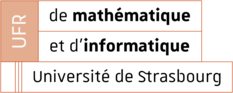
\includegraphics[scale=1.]{img/logo_UFR_2.png}}
\end{figure}

\pagenumbering{roman}

\newpage
% \addcontentsline{toc}{section}{Table des matières}
\renewcommand{\contentsname}{Table des matières}
\tableofcontents

\newpage
\addcontentsline{toc}{section}{Liste des figures}
\renewcommand{\listfigurename}{Liste des figures}
\listoffigures

\newpage
\pagenumbering{arabic}
\vspace*{0.01cm}
\section*{Introduction}
L'objectif du projet est de réaliser un système de recherche d’information dans une collection de descriptions de films publiées sur Allociné.\\
Le projet se décompose en deux parties:
\begin{itemize}
\item  Prédiction du genre des films par TAL
\item Visualisation des résultats
\end{itemize}

L'ensemble des fichiers (jeux de données et notebooks) utilisés sont accessibles sur GitHub: \url{https://github.com/FABallemand/ProjetTAL}

\newpage
% \vspace*{0.01cm}
% \input{src/sampling.tex}

% \newpage
% \input{src/evol.tex}

% \newpage
% \input{src/gen.tex}

\newpage
\vspace*{0.01cm}
\section*{Conclusion}
Avec le temps et la puissance de calcul à disposition, le meilleur modèle pour
la classification des films semble être le réseau neuronal convolutif. Il offre
des résultats proches du BILSTM pour un temps d'entraînement significativement
plus faible.

\begin{table}[]
    \begin{tabular}{|l|l|l|l|l|}
        \hline
        Modéle    & Radom Forest & CNN     & BILSTM  & Transformer \\
        \hline
        Précision & 66\%         & 72.91\% & 74.51\% & ???         \\
        \hline
    \end{tabular}
    \caption{Résultats des modèles testés}
    \label{accuracy}
\end{table}

En entrainant le même modèle avec l'ensemble des données du jeu d'entraînement et en testant sur l'ensemble des données du jeu de test, on observe une précision d'environ 50\%.\\
Ce niveau de précision semble faible, cependant si on observe le vecteur de probabilités à la sortie des couches denses, dans 80\% des cas le CNN place le genre attendu dans les trois premiers genres prédits (et il semble faire des erreurs sur les genres qui sont proches par exemple \textit{science-fiction} et \textit{historique} sont rarements ensembles dans les trois premires genres).

Les résultats obtenus avec le modèle choisi ne sont peut-être pas les meilleurs résultats qu'il est possible d'obtenir sur ces jeux de données. Voici quelques pistes de recherche que nous aurions aimé explorer:
\begin{itemize}
    \item Transformer
    \item Grid search avec différents pré-traitement des données (tokénisation, vectorisation...) sur les différents modèles
    \item Méthodes d'intelligence collective (exemple: entraîner plusieurs CNN et efffectuer un vote pour prédire le genre)
\end{itemize}

Après avoir enregistré les prédiction dans un fichier au format \textsf{csv}, les résultats obtenus peuvent être parcourus et analysés au moyen d'une interface web basée sur Solr \cite{solr}. L'utilisation des panneaux latéraux permet de filtrer les résultats des requêtes. (Figure \ref{solr})

\begin{figure}
    \center
    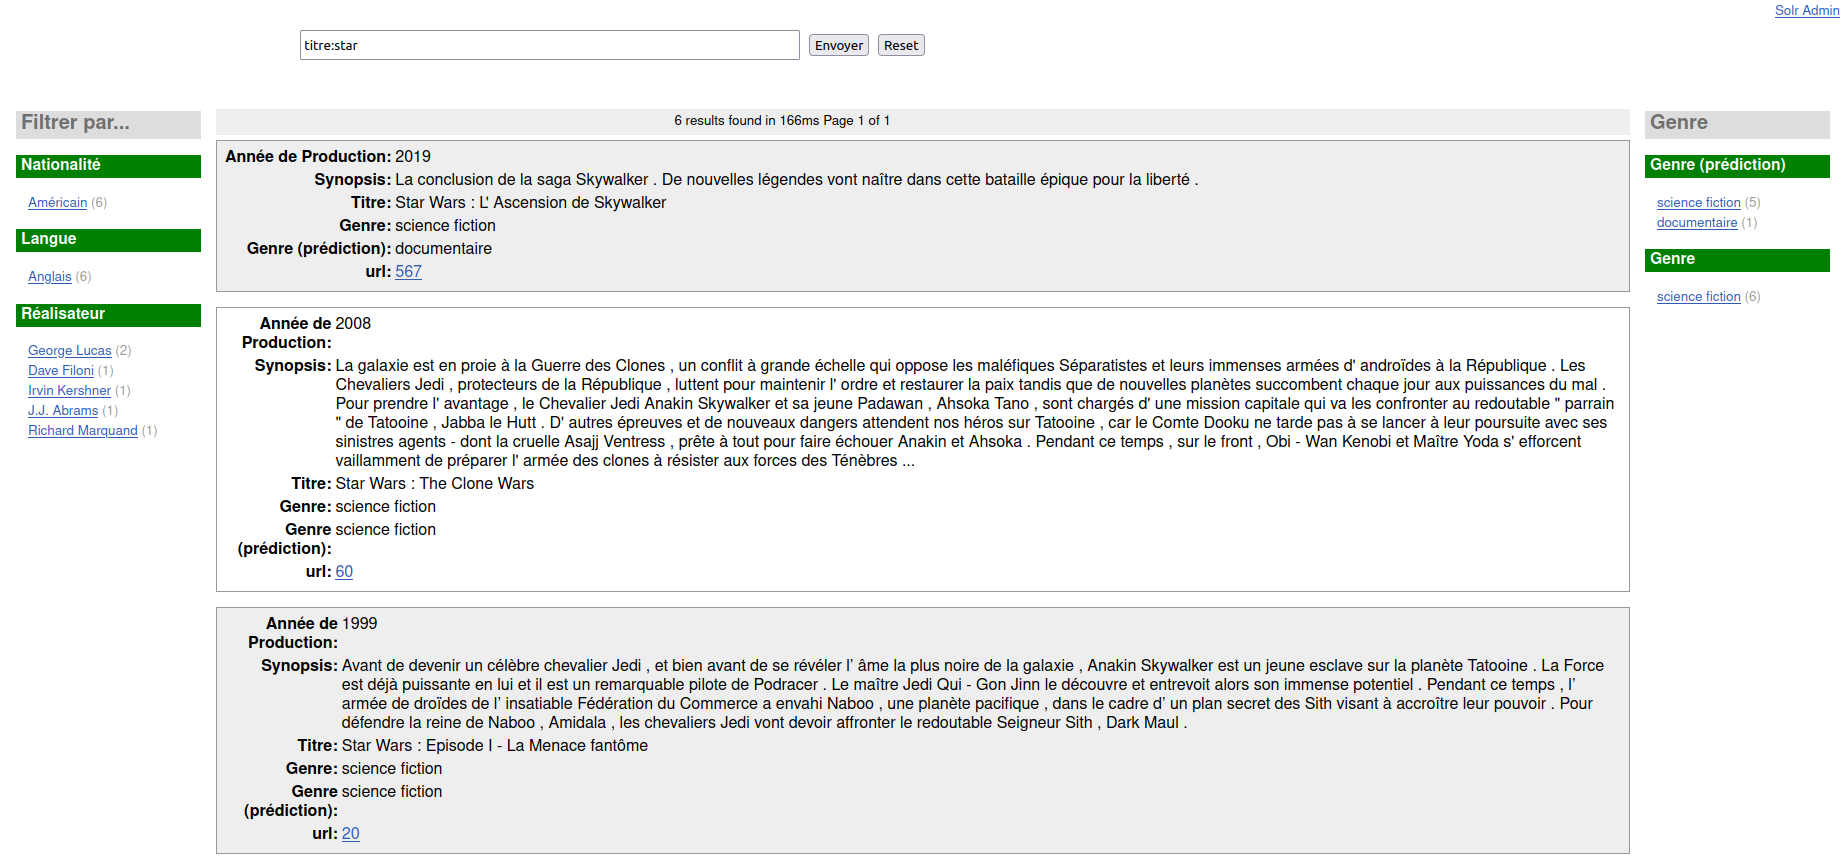
\includegraphics[scale=.25]{img/solr.png}
    \caption{Interface web Solr pour une requête sur le mot \textit{star}}
    \label{solr}
\end{figure}



\newpage
\addcontentsline{toc}{section}{Bibliographie}
\renewcommand{\refname}{Bibliographie}
\bibliographystyle{plain}
\bibliography{bibliographie}

\end{document}